\section{Introduction}

Text-conditioned image generation is processing longer texts, with a growth from 77 tokens in Dall-E~\cite{dalle} to 300 in PixArt-$\alpha$~\cite{pixarta}, and recently achieving 2,000-token capacity in autoregressive models~\cite{chameleon}. 
In this regard, generating comprehensive and controllable images with longer text input, such as images with complex layout or dense text, is considered a promising testbed.


% Text-conditioned image generation is processing inputs of longer texts, with a growth in processing inputs of longer contexts from 77 text tokens in Dall-E~\cite{dalle} to 300 text tokens in PixArt-$\alpha$~\cite{pixarta}, and recently achieving 2,000-token capacity in autoregressive architectures~\cite{chameleon}.
% In this regard, the task of generating comprehensive and controllable images with longer text input, such as image with complex layout or dense text, is considered a promising testbed.


Text plays a central role in image generation, serving as one of the most pervasive elements in visual communication through news, books, advertisements, and more. 
For instance, over 50\% of images in LAION-2B~\cite{laion} contain text~\cite{parrot}. 
However, despite the increasing prevalence of dense text in real-world scenarios, state-of-the-art models such as LlamaGen~\cite{llamagen}, Chameleon~\cite{chameleon}, and TextDiffuser2~\cite{textdiffuser2} struggle with tasks requiring the generation of long and complex text. 

% Text plays a central role in image generation, serving as one of the most pervasive elements in visual communication through news, books, advertisements, and more. 
% For instance, over 50\% of images in image generation datasets LAION-2B~\cite{laion} contain text~\cite{parrot}. 
% However, despite the increasing prevalence of dense text in real-world scenarios, state-of-the-art models such as LlamaGen~\cite{llamagen}, Chameleon~\cite{chameleon} and TextDiffuser2~\cite{textdiffuser2} struggle with tasks requiring the generation of dense text. 
% However, despite the increasing prevalence of dense text in real-world scenarios, state-of-the-art models such as SD-XL3~\cite{sd3}, DallE-3~\cite{dalle3} and Chameleon~\cite{chameleon} struggle with tasks requiring the generation of dense text. 


This limitation stems from the reliance on existing text-rich image datasets like Marion10M and AnyWords3M~\cite{anytext,textdiffuser2}, which focus on short and simple text, failing to meet the demand for handling longer and more intricate inputs. 
Such limitations are particularly evident in practical scenarios, ranging from advertising layouts that require seamless brand messaging integration to infographics that demand precise synchronization of text and visuals, as shown by the Notice Board in Figure~\ref{fig:motivation}.

\begin{wrapfigure}{r}{0.45\textwidth}
    \centering
    \vspace{-1.5em}
    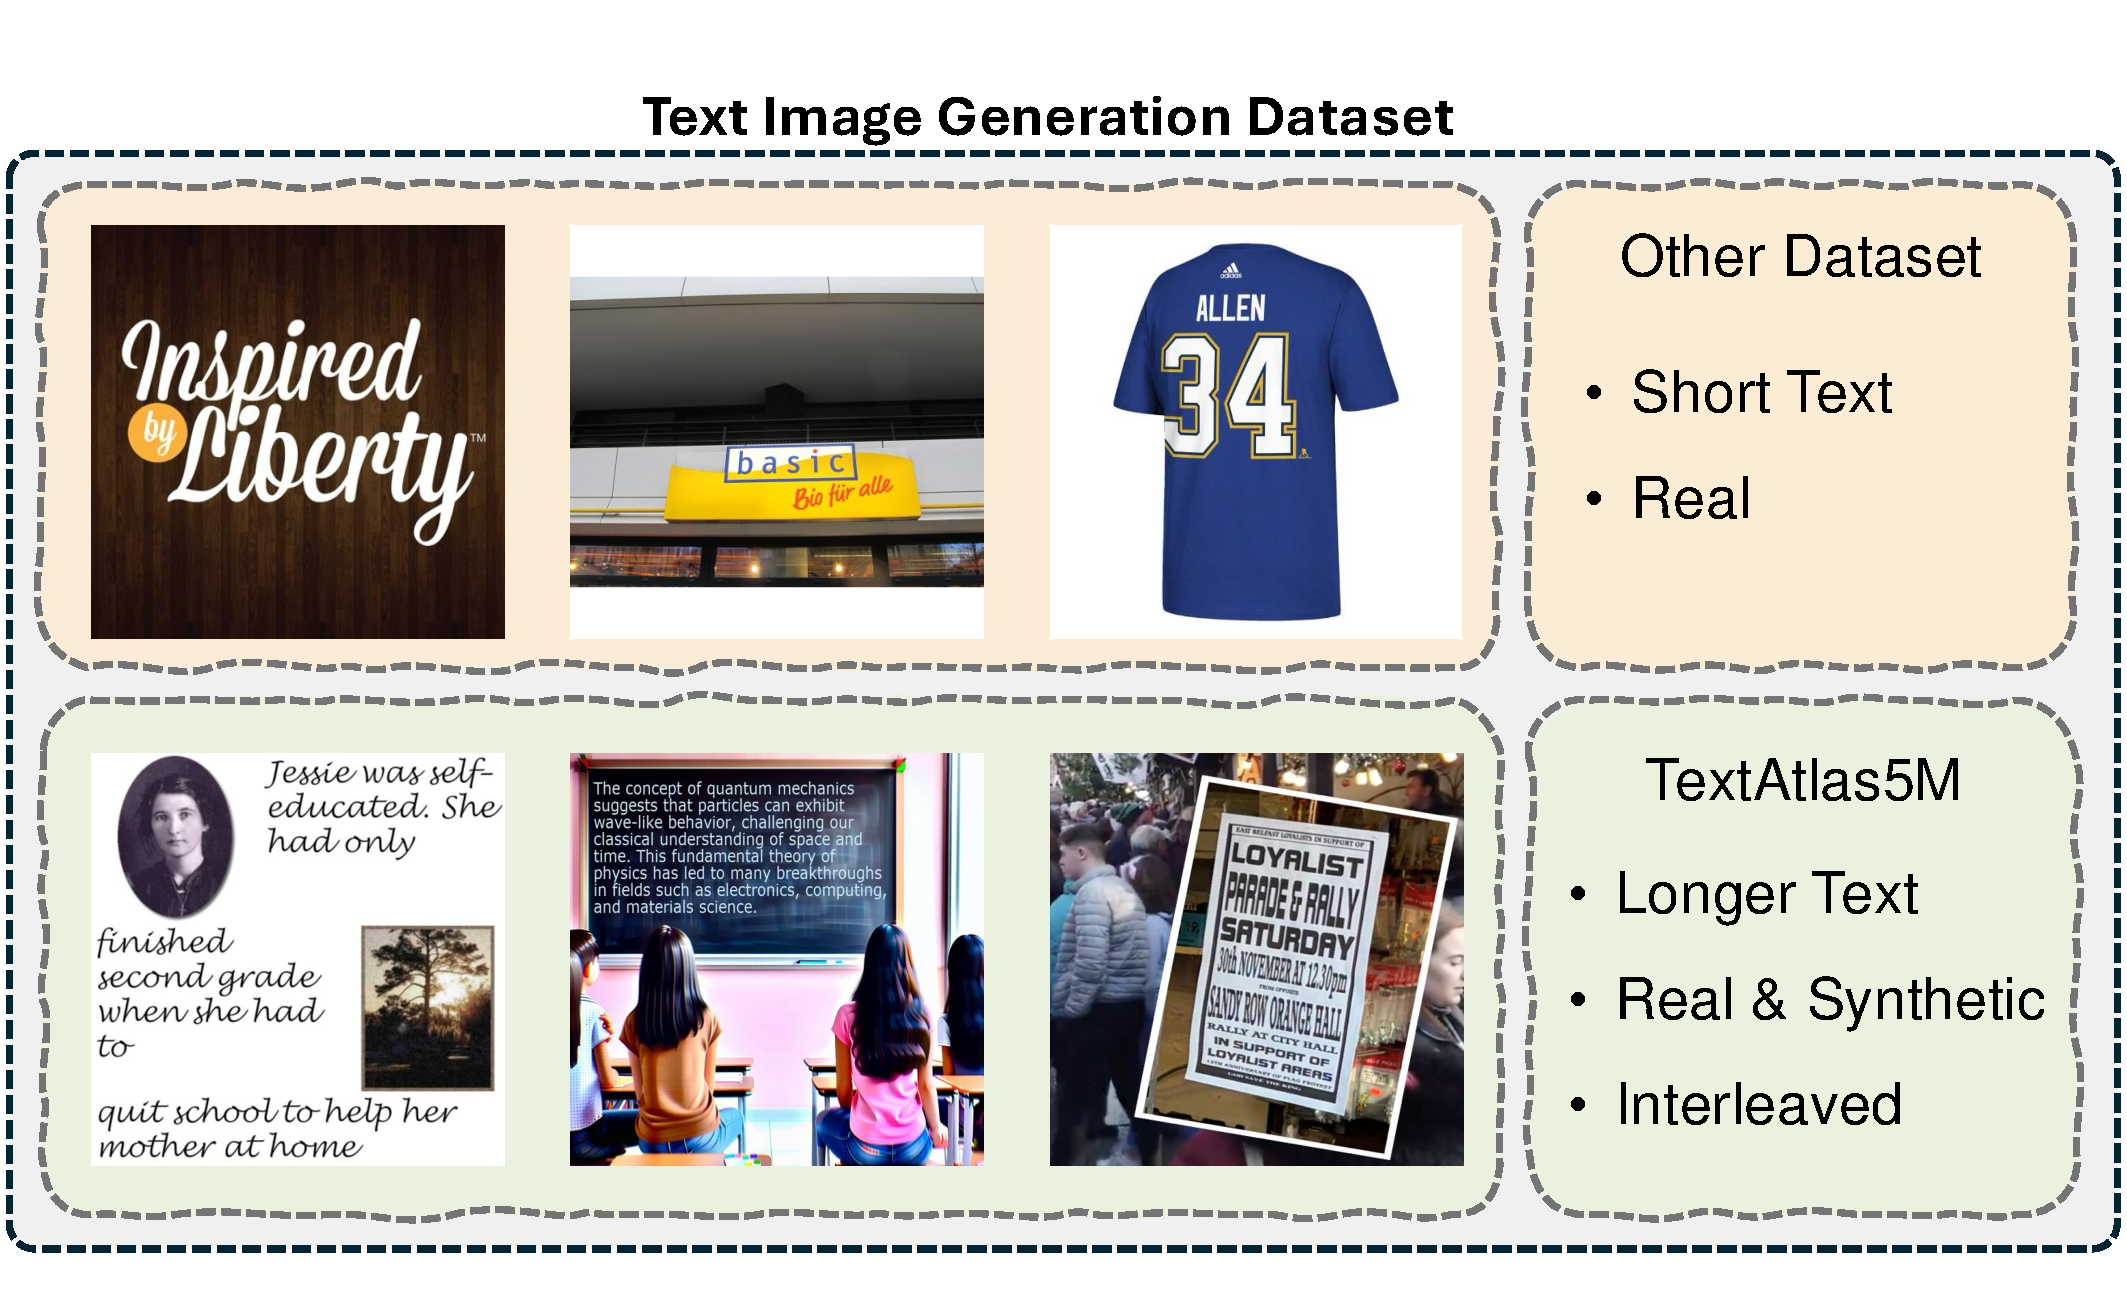
\includegraphics[width=0.44\textwidth]{figures/src/fig1_v1.pdf}
    % \vspace{-1.5em}
    \caption{
    \textbf{Comparison of \DatasetName~ with previous datasets.}  
    \DatasetName includes more diverse and complex long-form text than prior short-text datasets~\cite{laion,anytext,textdiffuser}.
    }
    \label{fig:motivation}
    \vspace{-1em}
\end{wrapfigure}

% \begin{figure}
%     \centering
%     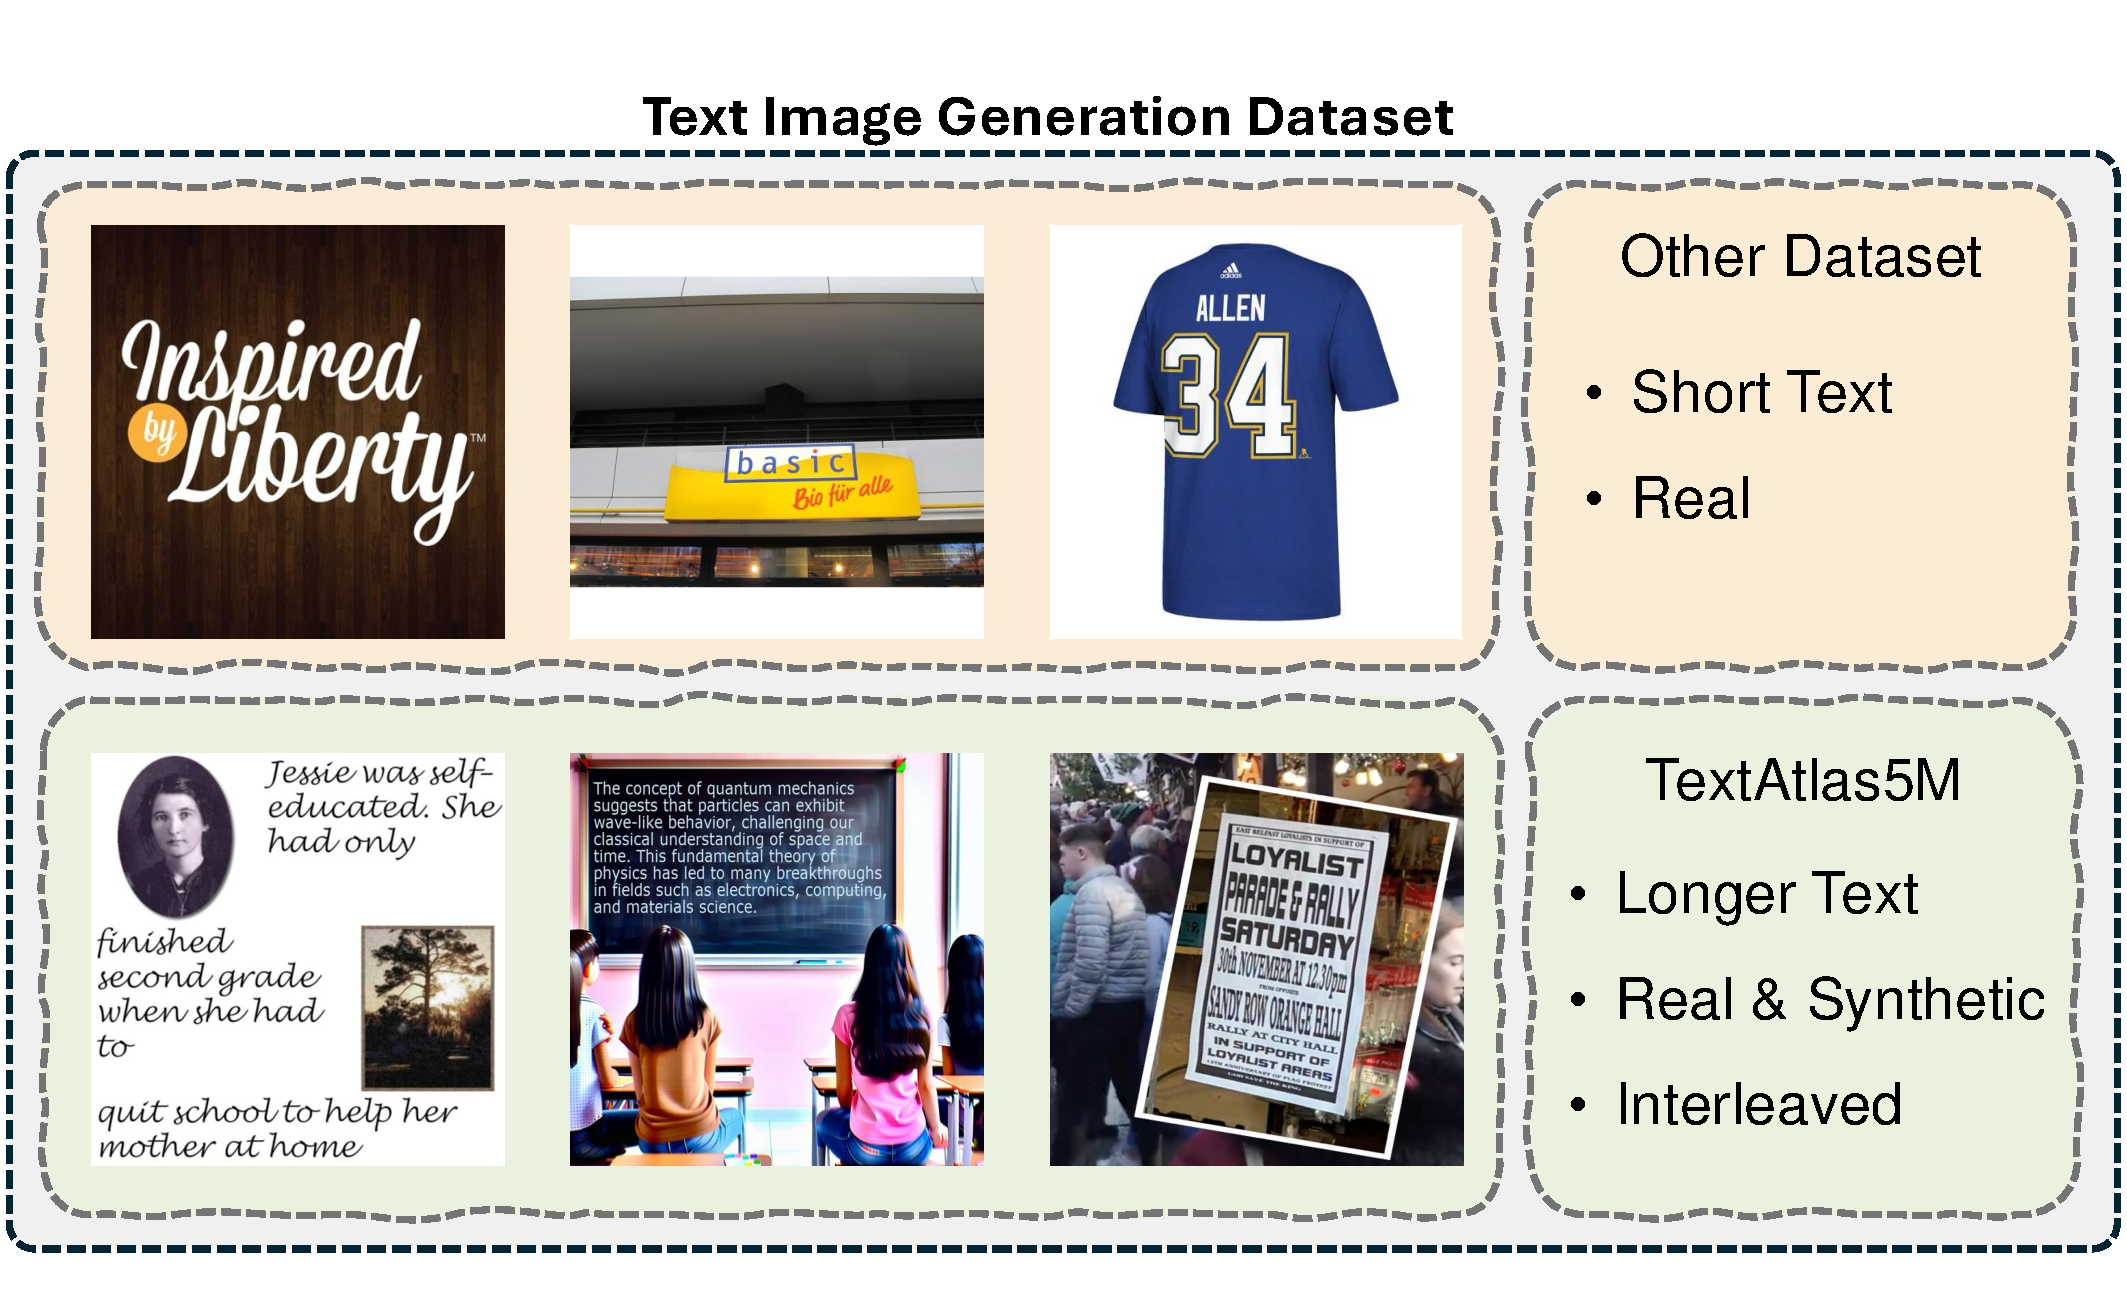
\includegraphics[width=.8\linewidth]{figures/src/fig1_v1.pdf}
%     \caption{
%     \textbf{A comparison of \DatasetName~ with previous text-rich image datasets~\cite{laion,anytext,textdiffuser}.}  
%     Unlike prior datasets with short text, \DatasetName features more diverse, complex long-form text.
%     }
%     \label{fig:motivation}
% \end{figure}



To address these challenges, we introduce \DatasetName, a comprehensive dataset designed to advance and evaluate text-to-image generation models, with a particular focus on generating dense-text images. 
As illustrated in Figure~\ref{fig:motivation} and Table~\ref{tab:dataset_comparison}, \DatasetName stands out in several key ways compared to previous text-rich datasets. 
Unlike earlier datasets, which primarily focus on short and simple text, \DatasetName includes a diverse and complex range of data. 
It spans from interleaved documents and synthetic data to real-world images containing dense text, offering a more varied and challenging set of examples. 
Moreover, our dataset contains longer text captions that pose additional challenges for models, and incorporates human annotations on difficult cases to ensure a more rigorous evaluation.
% Moreover, our dataset features longer text captions, which pose additional challenges for models, and includes human annotations for particularly difficult examples, ensuring a more thorough evaluation of model capabilities.

The synthetic subset progresses through three levels of complexity, starting with simple text on clean backgrounds. 
It then advances to interleaved data, blending text with visual elements, and culminates in synthetic natural images, where realistic scenes integrate seamlessly with text.
The real image subset captures diverse, real-world dense-text scenarios. 
It includes filtered samples from datasets like AnyText~\cite{anytext} and TextDiffuser~\cite{textdiffuser}, detailed descriptions from PowerPoint slides, book covers, and academic PDF papers. 
To enrich diversity, we also gather dense-text images guided by predefined topics from CommonCrawl~\cite{commoncrawl} and LAION-5B~\cite{laion}.
To assess the capability of model in dense text image generation, we introduce a dedicated test set, \EvalDatasetName, designed for comprehensive evaluation. 
This test set spans four distinct data types, ensuring diversity across domains and enhancing the relevance of \DatasetName~for real-world applications. 
Our contributions are threefold: 

\ding{172} We introduce \DatasetName, \textbf{the first large-scale dataset specifically designed for long-text image generation}, which combines three levels of synthetic data with diverse real-world images covering dense-text scenarios across multiple domains. 
\ding{173} \EvalDatasetName fill the gap in assessing long-text rendering quality, requiring models to accurately process and generate extended textual content, thus going beyond existing benchmarks. 
\ding{174} We conduct comprehensive evaluations of both proprietary and open-source models, revealing significant challenges in long-text generation and highlighting limitations of current approaches. 
In particular, we fine-tune \textbf{both diffusion and autoregressive models} on \DatasetName, achieving consistent improvements in text rendering and demonstrating the  utility  of \DatasetName for advancing future research on text-rich image generation.

% Our contributions are as follows: 
% \begin{itemize}
% \item \textbf{First Large-Scale Dataset for Long-Text Image Generation:}  
% We introduce \DatasetName, the first large-scale dataset specifically designed for long-text image generation. 
% It includes three levels of synthetic data and a diverse collection of real-world images, spanning a wide range of dense-text scenarios across multiple domains.

% \item \textbf{Long-Text Evaluation Benchmark:}  
% We design a dedicated test set to address the longstanding gap in metrics for evaluating long-text information in image generation. By requiring models to effectively process and generate longer text, \DatasetName sets itself apart from existing text rendering benchmarks.

% \item \textbf{Comprehensive Model Evaluation:}  
% We thoroughly evaluate proprietary and open-source models to assess their long-text generation capabilities. 
% The results reveal the significant challenges posed by \DatasetName and provide valuable insights into the limitations of current models, offering key directions for advancing text-rich image generation in future research.
% In particular, we fine-tune two autoregressive models (1B and 7B) on our dataset and observe consistent and significant improvements in text rendering, underscoring the utility of this dataset for model training.
% \end{itemize}


\input{tables/dataset_comparison}

